%
% ---------------------------------------------------------------
% template para escribir tesis/memorias en
% la Universidad Diego Portales
% ---------------------------------------------------------------
%
\documentclass[final]{udpthesis}

\usepackage[T1]{fontenc} % output
\usepackage[utf8]{inputenc}% input
\usepackage{lmodern}
\usepackage{graphicx}

\usepackage{amsmath}

\usepackage{amsmath} %%% para split
\udptheme{EIT}


% ---------------------------------------------------------------
% Comienzo del documento
% ---------------------------------------------------------------
\usepackage{hyperref}
\hypersetup{%
    pdfborder = {0 0 0}
}
%\usepackage[numbered]{bookmark}
\begin{document}
\frontmatter
\title{Propuesta de descriptor basado en partes para el reconocimiento de expresiones y objetos en secuencias de imágenes}
\author{Rodrigo Andrés Fuenzalida Cabeza}
\date{Junio, 2014}% (Ej: Enero, 2006)

\professor{Adín Ramírez}
\committee{Javier Pereira}{}
\dedicatory{Este trabajo va dedicado a mi madre, por todos esos años de sacrificio para darme una excelente educación.}
\acknowledgment{(Nota redactada sobriamente en la cual se agradece a quienes han colaborado en la elaboración del trabajo.)}
\makecover


% Indices de materia, figuras y tablas
\tableofcontents                        % tabla de contenido
\listoffigures                          % índice de figuras
\listoftables                           % índice de tablas

% Resumenes
\begin{abstract}
(Abstract es el resumen en inglés que no debe exceder una página.)
\end{abstract}

\begin{resumen}
(El resumen no debe contener menos de 100 palabras ni mas de 300 palabras.)
\end{resumen}


% Contenido
\mainmatter
\chapter[Introducción]{Introducción}\label{ch:capitulo1}
%\fpar
En este capítulo pasaremos a revisar las bases del problema que estamos planteando, con el fin de dar a conocer nuestra motivación, el contexto del problema y a su vez presentar los objetivos generales y específicos de nuestra investigación.

% ANTECEDENTES Y MOTIVACION

\section{Motivación}\label{chsub:Motivación}

Como consecuencia de las nuevas tecnologías de comunicación y al uso masivo de Internet en la sociedad actual, la cantidad de información audiovisual disponible en formato digital está alcanzando cifras realmente elevadas. Es por ese motivo que ha sido preciso diseñar sistemas que nos permitan describir el contenido de varios tipos de información multimedia para poderlos buscar y clasificar. 

Nuestra principal motivación es poder generar un descriptor (Definición~\ref{def:desc}) eficiente, en tiempo de ejecución y que sea ligero, además de aportar nuevos conocimientos y nuevas opciones al estado del arte actual. La importancia de este estudio es poder generar contenido que sea utilizado posteriormente como base para nuevas investigaciones. En detalle, nuestra propuesta nos motiva a preparar un estudio digno de ser publicado y usado como referencia. Además, hoy en día y con los avances tecnológicos realizados a la fecha, es inevitable no querer abordar desafíos relacionados con la detección y reconocimiento de objetos y personas. Algunos ejemplos los podemos ver en las propuestas realizadas por Google, el que con tan solo subir una imagen, nos entrega un sin fin de imágenes que tienen relación con la imagen de entrada, o Facebook el cual detecta automáticamente los rostros de personas, y ni pensar lo que pueden llegar a hacer. Quizás en un futuro, incluso detecten que estás en cierto lugar, con tan solo analizar el contenido de una imagen en la que apareces. Diversos son los posibles trabajos que se pueden hacer en esta área. Es así como estos dos grandes de la tecnología nos motiva a crear nuestra propia propuesta para hacer cosas novedosas y que llamen la atención de las personas.

\section{Problema}\label{sec:problema}
Hoy en día el mayor problema es poder obtener una representación fiel de un objeto o una expresión facial, es por esto que nos ha llamado mucho la atención distintas técnicas que resuelven este problema y es por ello que hemos decidido presentar nuestro propio algoritmo para describir distintos objetos y a su vez expresiones faciales. El objetivo, es que este algoritmo sea rápido y eficiente, tratando de obtener una precisión alta con respecto al estado del arte.

\section{Contexto}\label{sub:Contexto}

Hoy en día es habitual escuchar a las personas comentar sobre las cosas que hace Facebook o Google en el campo de visión por computador, por ejemplo, Facebook reconoce los rostros de las personas y te recomienda etiquetarlos o te dice ``esta persona puede ser conocido tuyo'' por medio de una fotografía, ó como ``Google Image'' que con tan solo escribir una palabra, éste te entrega un conjunto de imágenes extraídas de la web relacionadas con la palabra escrita, estos ejemplos despertaron gran interés en nosotros, por lo que nos aventuramos a explorar esta área de la informática.

Presentaremos una manera eficiente, ligera y rápida para la identificación de objetos y expresiones faciales. El objetivo principal es que nuestra propuesta sea los suficientemente ligera para poder ser utilizada en dispositivos móviles, la finalidad, por ejemplo, es pasear por un museo y dentro de este, visualizar un elemento; y mientras lo observamos obtenemos información sobre este mismo de forma rápida y precisa, incluso poder ir por la calle, ver a personas y poder saber quienes son antes de que nos saluden, detectar objetos interesantes y obtener información sobre ellos, llevar la computación más allá del viejo y olvidado ordenador.

Nos centraremos en la investigación de un nuevo mecanismo de descripción de características con el fin de crear una estructura que represente eficazmente dichas características y sea ligero para su procesamiento en el reconocimiento de objetos y expresiones.

\section{Objetivos}
La idea principal es generar un descriptor basado en partes utilizando métodos de reconocimiento de patrones temporales.
\begin{itemize}
		\item Objetivos generales:
			\begin{itemize}
				\item Combinar los diferentes métodos para generar un nuevo descriptor.
				\item Analizar técnicas basadas en partes y basadas en apariencia, tanto para objetos como para expresiones faciales en secuencia de imágenes.
			\end{itemize}
		\item Objetivos específicos:
			\begin{itemize}
				\item Analizar y evaluar el comportamiento del descriptor con conjuntos de imágenes, para poder obtener métricas que nos permitan identificar que tan buena es nuestra propuesta para identificar objetos.
				\item Analizar y evaluar el comportamiento del descriptor con diversas imágenes, para poder obtener métricas que nos permitan identificar que tan buena es nuestra propuesta con expresiones faciales.
				\item Analizar la precisión del descriptor, es decir, obtener métricas que nos permitan verificar mediante experimentos que tan eficiente es el algoritmo propuesto.
				\item Analizar el rendimiento y velocidad de computo de nuestra propuesta con métricas especificas para analizar dicho comportamiento.
				
			\end{itemize}			

	\end{itemize}

\section{Solución propuesta}

Nuestro trabajo propone mejorar el trabajo de Felzenszwalb et al.~\cite{Felzenszwalb2010}, utilizando como medio el marco de desarrollo creado por el grupo de trabajo de D. Ramanan. Esto nos ayudará a crear y probar nuestro algoritmo, con el fin de hacer una comparación entre lo presentado en el estado del arte (ver Sección~\ref{ch:capitulo2}) por Felzenszwalb. En concreto, crearemos un algoritmo para representar objetos reales de tal forma que este proceso sea más rápido y eficiente en el sentido de obtener mejores resultados que lo presentado en Felzenszwalb et al.~\cite{Felzenszwalb2010}.

\section{Resultados esperados}
Esperamos poder crear un nuevo descriptor robusto con ayuda de los trabajos hechos con anterioridad relacionados con este tema para poder identificar tanto objetos como expresiones. Diseñaremos nuestros algoritmos con el fin de generar un descriptor eficiente (con la idea de que pueda ser utilizado en un sistema móvil), para así ayudar a las personas a obtener información del mundo real de forma más fácil y dinámica.

A su vez queremos analizar y verificar que nuestra propuesta cumple con los estándares vistos en el estado del arte de nuestra investigación, para así proponer nuestro método como, un método robusto y eficiente en comparación con los que existen en la actualidad.

\section{Resumen}
En este capítulo revisamos los antecedentes personales que nos motivan a realizar esta investigación, en los capítulos posteriores pasaremos a revisar el estado del arte (Capítulo~\ref{ch:capitulo2}), algunas definiciones preliminares (Capítulo~\ref{ch:capitulo3}); En el Capítulo~\ref{ch:capitulo4} pasaremos a revisar el marco de desarrollo construido por el grupo de trabajo de D. Ramanan, el cual nos permitirá probar nuestra propuesta. Luego en el Capítulo~\ref{ch:capitulo5} presentaremos nuestra solución al problema propuesto, para finalmente en el Capítulo~\ref{ch:capitulo6} revisar los resultados obtenidos tanto para objetos como para expresiones faciales.
\chapter[Trabajos relacionados ]{Trabajos relacionados }\label{ch:capitulo2}

En el área del reconocimiento de patrones, visión por computadora, es un área que posee muchos estudios~\cite{survey2005}. Es por esto que en este capítulo pasaremos a revisar diversas técnicas y algoritmos. Una de las ideas básicas de estos algoritmos es que sean capaces de recibir una imagen como entrada y crear una representación que describa al(los) objeto(s) que estén presentes en dicha imagen. Esta sección comprende el detalle de las técnicas de detección y reconocimiento, tanto para objetos como para expresiones faciales. Si bien esta área es extensa, trataremos de abarcar aquellas investigaciones que sean un aporte y nos ayuden a crear las bases para nuestro trabajo.

% SECCION DE DETECCION 
\section{Detección y reconocimiento}
La detección de objetos es una tarea ardua que ha sido estudiada durante décadas, esto se puede ver en el estudio que resumen 50 años de investigaciones relacionadas con el reconocimiento de objetos~\cite{Andreopoulos2013}. El fin de detectar objetos, es lograr obtener una representación fiel del objeto que se quiere detectar, extrayendo así, por ejemplo, sus características únicas que posteriormente será utilizada para su reconocimiento y clasificación.

En cuanto al reconocimiento se han realizado estudios en dos contextos: objetos rígidos en 2D y 3D\@. El objetivo principal del \textit{reconocimiento de objetos}, es poder clasificar de forma correcta las clases que se están observando. A modo de ejemplo, en una escena donde hay siete perros y tres gatos, el objetivo del algoritmo que se utilice es que identifique con el menor error posible que los siete perros que hay en una escena sean perros y lo mismo para los tres gatos.

En otras áreas de la detección y el reconocimiento, el reconocimiento de caracteres, que en los últimos años ha sido campo de estudio, es un caso de estudio muy interesante dada la naturaleza de su información, ya que ésta es más acotada. 

\subsection{Modelo}
\label{subsec:modelo}
Un modelo es una abstracción teórica del mundo real, que nos permite representar la información de forma simplificada con el objetivo de realizar predicciones con los datos necesarios. Estos modelos permiten encontrar \textit{igualdades o similitudes} en los datos. Más en concreto, se suele entrenar un modelo con un conjunto de datos que representan una clase, para luego usar esta representación para predecir nuevos datos de entrada. En cuanto a la detección y reconocimiento de objetos, se utilizan modelos llamados descriptores, los cuales son algoritmos que extraen características más representativas de una imagen. 

\begin{definition}[Modelos estadísticos]
Estos modelos permiten representar situaciones cotidianas en forma matemática, lo que nos permite tener una abstracción más exacta de sucesos cotidianos.
\end{definition}
 
\begin{definition}[Descriptor]

\end{definition}


\subsection{Modelos de detección y reconocimiento de objetos}
Torres-Méndez et al.~\cite{trsi2000}, presenta un modelo de reconocimiento de objetos, que es invariante a la posición de éste, a su rotación y su escala. Se presenta un algoritmo que en primera instancia, pre-procesa los datos, con el fin de normalizar los momentos de inercia que posee el objeto, extrayendo así las características topológicas del objetos. En una segunda fase, reconocimiento es logrado usando el algoritmo, \textit{Holographic Nearest-neighbor (HNN)}. El principal motivo por el cual se utiliza este algoritmo es su rapidez~\cite{trsi2000}, ya que a diferencia de otras arquitecturas de redes neuronales, este algoritmo es bastante rápido según Torres-Méndez et al.~\cite{trsi2000}. En general \textit{Holographic Nearest-neighbor}, posee un mejor desempeño al momento de reconocer, a diferencia de técnicas como \textit{Nearest-neightbor (NN)}. El algoritmo \textit{Holographic Nearest-neighbor} es similar al algoritmo \textit{Nearest-neightbor}, este algoritmo está basado en la idea de utilizar la mínima distancia euclidiana entre el dato de entrada y todos los vectores de entrenamiento. Además, para evitar la predominancia de algunos sub-grupos de características, el algoritmo \textit{Nearest-neightbor} normaliza las características. Esta normalización consiste en extraer el promedio de los vectores de características y dividirlo por la desviación estándar de cada una de las características presentes en el conjunto de datos de entrenamiento.

Amit~\cite{Amit2002}, presenta técnicas como: \textit{Searching correspondence space}, el cual realiza una búsqueda sistemática, para el conjunto de características locales de la imagen. En este caso los emparejamientos deben satisfacer ciertas restricciones. Restricciones únicas implican una relación directa entre las características del modelo y las características de la imagen. Restricciones binarias implican la relación entre un par de características del modelo y de un par de características de la imagen. Diversas técnicas basadas en heurísticas de árboles se emplean para encontrar los diversos emparejamientos, con el fin de encontrar el emparejamiento óptimo de estas características. A su vez, se presentan varios modelos para reconocimiento de objetos, muchos de ellos utilizados por estudios realizados en esta área. Por ejemplo, \textit{Deformable-Template Models}, representa las características de un objeto, utilizando un modelo estadístico (ver Sección~\ref{subsec:modelo}), el cual describe la variabilidad que posee una instancia de un objeto en términos de una probabilidad a priori. Además, una representación  estadística de la imagen, entrega una particular deformación de la porción del objeto analizado. La combinación de ésta representación y la probabilidad priori, definen una distribución posterior de la deformación que posee la imagen.

Lowe~\cite{sift2004} presenta un método para la extracción de características invariantes de una imagen que son utilizadas para hacer una comparación entre diferentes vistas o escenas de un objeto. Las características son invariantes a la escala de la imagen y la rotación que esta pueda presentar. Los descriptores, estos se representan con la dirección y el gradiente que poseen los puntos de interés encontrados en etapas previas, luego se preprocesan los datos con una función de peso gaussiana, la cual asigna un peso a cada uno de los puntos. El propósito de este filtro es evitar que las muestras sufran variaciones.

En Bernstein~\cite{statistical2005}, se propone un modelo denso y con un rendimiento que otorga una tasa de clasificación alta, este modelo consiste en en una mejora a los modelos \textit{Sparse}, descritos por Amit~\cite{Amit2002}. este modelo usa mezcla de partes que definen a un nivel medio características locales basándose en orientaciones binarias en los bordes de los datos de entrada. Este estudio probó su modelo en un conjunto acotado de caracteres escritos a mano, además, se probó en y entreno para poder detectar distintos lados de automóviles.

Bay et al.~\cite{surf2008} presenta un detector y descriptor que es invariante a las rotaciones, llamado \textit{Speeded-Up Robust Feature (SURF)}. SURF utiliza un descriptor basado en distribuciones. Para SURF la creación de un descriptor debe ser único e invariante al ruido, para esto cada descriptor describe una distribución de intensidad de los puntos adyacentes al punto de interés, similar a lo que se postula en Lowe~\cite{sift2004}, pero con la diferencia que no se utiliza el gradiente sino que una distribución de primer orden basado en los wavelet the Haar.

Felzenszwalb et al.~\cite{Felzenszwalb2010} presenta un modelo basado en partes,  el cual utiliza varias partes de la imagen con el fin de determinar si existe un objeto de interés en ella. En este trabajo se busca optimizar \textit{Dalal-Triggs detector} el que utiliza \textit{Histogram of Oriented Gradients (HOG)}~\cite{hog2005} (ver Sección~\ref{subsec:hog}). Este tiene como principal objetivo obtener características específicas del objeto mediante la dirección de los gradientes o bordes, esto es implementado de la siguiente forma: Se divide la imagen en pequeñas porciones, llamadas celdas, las cuales generan otros histogramas de gradientes o bordes por cada pixel dentro de esta celda, combinando estos se obtiene la representación del descriptor. La mejora realizada sobre este método es que en paralelo se computa una función que maximiza los puntos obtenidos por HOG, lo cual permite capturar más características en el mismo rango de muestreo, este estudio será analizado con mayor detalle en el Capítulo~\ref{ch:framework}.

Choi et al.~\cite{treebased2012}, se propone un modelo basado en el contexto el cual maneja distintas combinaciones o locaciones de objetos que guía un detector el cual produce una interpretación semántica de la imagen que se está analizando. El objetivo de este trabajo es poder detectar múltiples categorías de objetos dentro de una misma escena. Por lo cual su modelo utiliza características globales dependientes entre las categorías de los objetos y las salidas locales de los descriptores utilizados.

\subsection{Modelos de detección y reconocimiento de expresiones}
Comúnmente existen dos enfoques para la extracción de características en el rostro: Basados en características geométricas y basados en apariencia, este último método utiliza filtros que crean características generales o en una área del rostro en especifico para crear características locales, con el fin de extraer los cambios de apariencia en la imagen del rostro.

Hsu et al.~\cite{Hsu2002} presentan un algoritmo de detección de rostros, como ellos mismos definen, un detector de rostros humanos juega un importante rol en aplicaciones actuales, es por esto que presentan un algoritmo de detección de rostro que trabaja con imágenes a color, tomando en cuenta distintas condiciones de luminosidad, así como fondos complejos. Dicho algoritmo funciona de la siguiente manera, primero, el algoritmo detecta las regiones donde está presente la piel, y luego genera un rostro candidato basados en la disposición espacial de estos parches cutáneos. Finalmente el algoritmo construye los ojos, boca y el mapa de los contornos, para verificar cada rostro candidato.

Ahone et al.~\cite{ahonen2006} presentan una representación eficiente del rostro, basándose en las características de las texturas extraídas por \textit{Local Binary Pattern (LBP)}. En primera instancia, la imagen es dividida en múltiples regiones donde es utilizado LBP para extraer las características locales de cada región, para luego ser representadas en un vector que contiene todas las regiones del rostro, el cual es utilizado como descriptor.

Ramirez et al.~\cite{ldnp2013} presenta un nuevo descriptor de características locales, llamado \textit{Local Directional Number Pattern (LDN)}, para reconocimiento de rostro y expresiones. Este estudio comenta que la eficiencia de un descriptor depende de su representación y la facilidad de extracción del rostro. Idealmente un descriptor debería tener una alta varianza con clases muy distintas (diferentes personas o expresiones), por otra parte si las clases son semejantes (misma persona o expresión), su varianza debería ser inferior o cero.

Ramanan y Zhu~\cite{Zhu2012} presentan un modelo unificado para detección de rostros, estimación de pose y estimación de contornos, este modelo está basado en una mezcla de árboles que comparten un un conjunto de partes. Se modela cada punto destacado como una parte y se usa una mezcla global para capturar los cambios topológicos de acuerdo al punto de vista que se está analizando. En este estudio se muestra como las técnicas de árboles pueden ser muy eficientes al momento de interpretar las partes que poseen los rostros.

\subsection{Resumen}
\chapter[Métodos ]{Métodos }\label{ch:capitulo3}

En este capítulo presentaremos una explicación detallada de diversos términos y métodos los cuales serán utilizados en capítulos posteriores. El objetivo principal es entregar un marco teórico, para simplificar las explicaciones que serán presentadas posteriormente. Es de vital importancia que estos conceptos queden explicados de forma detallada y clara, puesto que cumplen un rol fundamental en la construcción del método propuesto tanto por P. Felzenszwalb, como para nuestra futura propuesta.

\begin{definition}[Celdas]
\label{def:cel}
Una celda consiste en una región de la imagen que mide $8$ píxeles de alto por $8$ píxeles de ancho ($8 \times 8$).
\end{definition}

\begin{definition}[Bloques]
\label{def:blo}
Un bloque es una región de la imagen que corresponde a $2 \times 2$ celdas.
\end{definition}

\begin{definition}[Bins]
\label{def:bin}
Un histograma está compuesto por bins. Un bin es la representación de la cuantificación de un espacio. Generalmente, en el bin se cuenta la cantidad de elementos del espacio que existen en la región definida por dicho bin.
\end{definition}

\section{Histogram of Oriented Gradients}\label{subsec:hog}
\textit{Histogram of Oriented Gradients} (\textit{HOG}) presentado por Dalal y Triggs~\cite{hog2005}, es un descriptor de características utilizado en visión por computador y procesamiento de imágenes. Este algoritmo sirve para representar objetos (latas, botellas, autos, personas, rostros, etc.). En términos generales, HOG es una técnica que cuenta las ocurrencias de las orientaciones de los gradientes en partes específicas de una imagen. Este método calcula un espacio de celdas superpuestas con el fin de normalizar las muestras locales y aumentar la precisión.

HOG cuenta con ciertos pasos que se deben realizar para obtener el descriptor de una imagen, esto se puede ver en la Figura~\ref{fig:hog_procedure}, y a continuación detallamos las etapas que componen el algoritmo HOG.

\begin{figure}[tb]
 \centering
  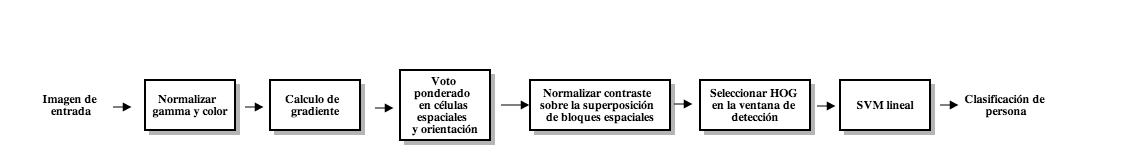
\includegraphics[width=0.8\textwidth]{Figuras/hog-procedure.png}
  \caption[Procedimiento de cálculo de HOG]{Procedimiento de cálculo de HOG.}
  \label{fig:hog_procedure}
\end{figure}

\subsection{Procedimiento de HOG}
Felzenszwalb et al.~\cite{Felzenszwalb2010} dividen la imagen en celdas (ver Definición~\ref{def:cel}), sin superposición (en la Figura~\ref{fig:blocks_cells} se puede apreciar la división de los bloques y las celdas antes descritas). Luego, por cada píxel dentro de una celda se acumulan los histogramas de orientación de gradientes. Estos histogramas capturan propiedades de forma local dentro de la celda. a su vez, estos histogramas son invariantes a pequeñas deformaciones.
El gradiente en cada píxel está discretizado en uno de los nueve contenedores (\textit{bins}) de orientación, y cada píxel vota por la orientación de su gradiente, con un valor que depende de la magnitud del gradiente. Para las imágenes en color, se calcula el gradiente de cada canal de color, eligiendo el canal con la mayor cantidad de píxeles donde la magnitud del gradiente esa mayor.

\begin{figure}[tb]
 \centering
  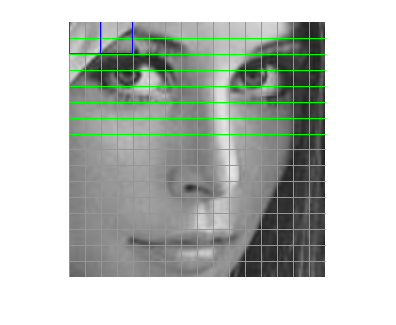
\includegraphics[width=0.5\textwidth]{Figuras/lena-grid.png}
  \caption[Bloques y celdas]{Bloque 1 (azul), bloque 2 (rojo), celdas (verde).}
  \label{fig:blocks_cells}
\end{figure}

Finalmente, cada histograma de las celdas es normalizado con respecto a la energía del gradiente en un vecindario alrededor de la celda. Se observan los cuatro bloques de $2 \times 2$ de celdas que contienen una celda particular, y luego se normaliza el histograma cada celda dada con respecto a la energía total en cada uno de estos bloques. Esto entrega un vector de longitud $9 \times 4$ que representa la información local de gradiente dentro de una célula.

\section{Pirámide}\label{sec:pyra}
La pirámide consiste en hacer varias iteraciones de una misma imagen con distintas resoluciones, donde en cada nivel de resolución se extraen las características más representativas con el descriptor de HOG\@. La Figura~\ref{fig:hog_pyra}, muestra los histogramas obtenidos luego de pasar una imagen por tres niveles de la pirámide, estos niveles son representados por $\lambda$ y en la fase de entrenamiento tienen un valor de 5, es decir, cinco niveles de profundidad~\cite{Felzenszwalb2010}.

\begin{figure}[tb]
 \centering
  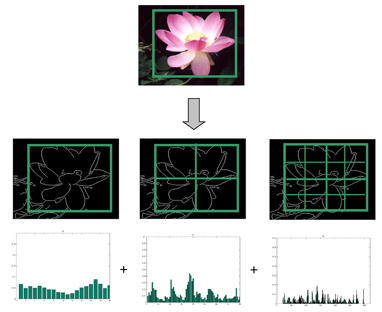
\includegraphics[width=1\textwidth]{Figuras/phog.jpg}
  \caption[Pirámide de HOG]{Pirámide de HOG~\cite{pyra}}
  \label{fig:hog_pyra}
\end{figure}

\section{Filtro y \textit{score}}\label{sec:fas}

\subsection{Filtro}
Un filtro está definido por una matriz de $w$ (ancho) por $h$ (alto) la cual define un vector de peso de $d$-dimensiones. Estos filtros especifican las características extraídas por HOG, en los niveles de la pirámide. El tamaño del filtro se crea en base a la razón entre el ancho $w$ y el alto $h$ de las imágenes, correspondientes al conjunto de datos que se está observando, es decir, en base a la proporción de los aspectos que tiene el conjunto de imágenes, donde los aspecto serán distribuidos por una distribución exponencial, en un rango definido entre -2 y 2 con una separación de 0.02. El área el filtro es calculado mediante el calculo de las áreas de las imágenes pertenecientes al conjunto de datos, de las cuales se extrae el 20\% de las imágenes ordenadas de forma descendente. Por último el tamaño del filtro es calculado como: $w = (area/aspecto)^2$ y $h = w*aspecto$.

\subsection{Score}
El \textit{score} de un filtro está definido por el producto punto entre su vector de pesos y las característica en la sub-ventana de la pirámide de HOG de dimensión $w \times h$. Esto es calculado mediante la convolución del filtro que se está analizando con la imagen correspondiente.
\section{SVM}\label{sec:lsvm}

\textit{Support Vector Machines} (\textit{SVM})~\cite{Vapnik1995, Duda2000, Cortes1995} es un tipo de algoritmo de aprendizaje supervisado que analiza información y reconoce patrones, utilizado para tareas de clasificación. Dado un conjunto de entrenamiento previamente etiquetado, por ejemplo en dos clases, SVM construye un modelo el cual es capaz de asignar una nueva muestra a una de las categorías previamente definidas, por lo que se define un clasificador binario lineal no-probabilístico.
SVM define un modelo como un conjunto de puntos en un espacio dado que representan un hiperplano en dicho espacio. Este hiperplano separa las clases con la mayor diferencia posible para clasificar sin problema dichas clases. Los nuevos datos que entren al modelo serán clasificados en una de las dos opciones de según el lado donde se encuentran respecto al hiperplano.

Además de realizar la clasificación lineal, SVM puede realizar de manera eficiente una clasificación no lineal utilizando el truco del \textit{kernel}, ver Sección~\ref{subsec:kernel_methods}.

\subsection{Ventajas de SVM}
\begin{itemize}
\item Eficiente en espacios de dimensiones altas.
\item Sigue siendo eficaz en los casos en que el número de dimensiones es mayor que el número de muestras.
\item Utiliza un subconjunto de puntos de entrenamiento en la función de decisión (llamada vectores de soporte), por lo que también es eficiente en el uso de memoria.
\item Versátil: diferentes funciones del \textit{kernel} pueden ser especificados para la función de decisión. \textit{Kernel} comunes se proporcionan, pero también es posible especificar \textit{kernels} personalizados.
\end{itemize}

\subsection{Desventajas de SVM}
\begin{itemize}
\item Si el número de características es mucho mayor que el número de muestras, el método probablemente entregue malos resultados.
\item SVMs no proporcionan directamente las estimaciones de probabilidad.
\end{itemize}

\subsection{Aplicaciones}
\begin{itemize}
\item SVM es útil en categorización de texto, esta aplicación puede reducir significativamente la necesidad de etiquetar instancias del conjunto de entrenamiento.
\item Clasificación de imágenes.
\item SVMs es útil en la ciencia médica para clasificar las proteínas con hasta un 90\% de los compuestos clasificados correctamente.
\item Reconocimiento de caracteres escritos a mano
\end{itemize}

\subsection{Kernel Methods}\label{subsec:kernel_methods}

Los métodos de \textit{Kernel} son un tipo de algoritmos utilizados en análisis y reconocimiento de patrones, los cuales son conocidos por ser utilizados en SVM~\cite{kernels}. La principal característica de estos métodos son sus diversos enfoques. Estos métodos representan la información en espacios de dimensiones mayores con el fin de poder separar las muestras, para así poder distinguirlas de manera más fácil. No existe una restricción para las dimensiones, pudiendo ser estas infinitas. Esta función de representación no necesita mayor complejidad de cálculo ya que existe una herramienta llamada, \textit{The} \textit{Kernel} \textit{Trick} la que simplifica esta tarea.

\subsection{The Kernel Trick}

\textit{The} \textit{kernel} \textit{trick} es una herramienta matemática que puede ser utilizada sobre algoritmos que únicamente utilicen el producto punto entre dos vectores. Donde sea que se utilice el producto punto de vectores se puede reemplazar por una función \textit{kernel}. Cuando la función \textit{kernel} es bien utilizada, permite que un algoritmo lineal pase a ser no-lineal, lo que logra cambiar el espacio de representación de los datos. Dependiendo del algoritmo esto puede representar un mayor esfuerzo tanto en el cómputo, como en su implementación. Los algoritmos no-lineales son equivalentes a su operador lineal original en el espacio de características $\varphi$.

\subsection{Propiedades de los Kernels}

Las funciones \textit{Kernel} deben ser continuas, simétricas y preferentemente deben tener una una matriz de Gram definida positiva~\cite{Gram}. \textit{Kernels} que satisfacen el teorema Marcer~\cite{minh2006mercer} están definidos semi-positivos, lo que significa que sus matrices no tienen valores propios negativos. El uso de un \textit{kernel} definido positivo asegura que el problema de optimización será convexo y la solución será única.

\subsection{Eligiendo el mejor Kernel}

Elegir el mejor \textit{kernel} dependerá mayormente del problema que se esté tratando de solucionar, dependiendo de las características del problema esto incluso puede llegar a ser una tarea tediosa y compleja. Como se mencionó anteriormente el \textit{kernel} que se utilice, dependerá exclusivamente de que es lo que queremos modelar. Un \textit{kernel} polinomial, por ejemplo, nos permite modelar conjuntos de características hasta el orden del polinomio. Funciones de base radial permite seleccionar los círculos o hiperesferas, a diferencia del un kernel lineal, que sólo permite crear líneas y hiperplanos.

El uso de un \textit{kernel} dependerá exclusivamente de la información que estemos extrayendo, siendo esta tarea algo que dependerá de quien esté realizando el desarrollo de una aplicación o algoritmo que use algún \textit{kernel} en específico.

\section{Resumen}\label{sec:resumen}

Cada uno de los conceptos revisados en este capítulo son de vital importancia para los capítulos posteriores, ya que son estos conceptos los que definirán parte de lo que presentaremos en las siguientes secciones. Esto forma las bases teóricas las cuales darán forma a nuestra propuesta. En nuestro caso es importante destacar el uso de HOG ya que es este algoritmo permite representar de cierta forma las imágenes procesadas, para luego poder clasificarlas con el uso de una variación de SVM, llamada \textit{Latent SVM} (el cual será explicado y detallado en el capítulo siguiente). Términos como \textit{filtro} y \textit{score} serán utilizados con regularidad ya que son estos los que definen porciones importantes del mecanismo de reconocimiento y detección para objetos y expresiones faciales de nuestra propuesta.



\chapter[Modelos basados en partes ]{Modelos para detección de objetos basados en partes discriminadamente entrenados }\label{ch:capitulo4}
En este capítulo se presenta un análisis extenso y exhaustivo al marco de desarrollo creado por Felzenszwalb y el grupo de desarrollo de D. Ramanan, el objetivo principal de este capítulo es presentar y analizar las partes que componen este marco, con el fin de entender su funcionamiento y así poder generar mejoras sobre este, tanto para generar los modelos, como para consumirlos en aplicaciones más ligeras. El uso de este marco de desarrollo está ligado a la simpleza de su uso y a su extremo potencial para generar modelos portables que pueden ser utilizados por otros lenguajes de programación. Cabe destacar que este marco de desarrollo fue creado en \textit{MATLAB}, lo que nos permite generar modelos con estructuras ligeras y que pueden ser utilizados por otros lenguajes de programación. En secciones posteriores discutiremos el contenido de este marco de desarrollo, a su vez discutiremos las ventajas y desventas de usar este programa.

\section{Marco de desarrollo}\label{sec:framework}
Para realizar el procesamiento del conjunto de datos se utiliza un marco de desarrollo creado por Felzenszwalb y el grupo de trabajo de D. Ramanan, el que nos permitirá generar los modelos para el reconocimiento de objetos. Este marco está basado en el conjunto de imágenes de la base de imágenes PASCAL~\cite{Everingham2010}. Como se mencionó anteriormente este marco está desarrollado en \textit{MATLAB}, con excepción de algunos archivos que fueron escritos en \textit{C} con el fin de poder hacer más rápido los procesos que tienen mayor complejidad de computo. Este marco nos permite generar modelos que luego pueden ser consumidos por distintos lenguajes de programación, convirtiendo a este programa en una herramienta de gran ayuda.

\subsection{Definición de datos}\label{sec:datos}
La definición de los datos es una etapa muy importante en este tipo de estudios, ya que esta etapa selecciona la información disponible para ser utilizada en etapas de entrenamiento y prueba. Esta etapa es la encargada de revisar y seleccionar los datos a ser procesados utilizando diversas especificaciones y formas de representación, para dar mejor uso y obtener mejores resultados con los datos de entrada. El preprocesamiento para el marco de desarrollo presentado en este estudio, se utiliza la base de datos PASCAL~\cite{Everingham2010}, la cual provee un conjunto de imágenes y anotaciones---más adelante explicado.

Se necesita detallar información específica de cada imagen, por lo que es necesario crear un archivo XML, con el mismo nombre de la imagen, que contenga la información necesaria para realizar el procesamiento, esto es llamado, anotación. La anotación especifica la clase de la muestra, la ruta del archivo; de dónde se obtuvo la imagen; entre otros atributos necesarios de las imágenes de entrenamiento. Lo más importante de estas anotaciones es que contiene la o las \textbf{regiones} de interés, dependiendo de cuántos objetos contenga la imagen. Una región, está representada por cuatro pixeles, los que a su vez, representan los vértices de una diagonal en un plano cartesiano, dónde su origen se encuentra ubicado en la esquina superior izquierda de la imagen. Es importante mencionar, que tanto el eje $x$ como el eje $y$, son positivos, por lo que cada pixel representa la distancia al origen, la forma de una región de interés se presenta en la Figura~\ref{fig:anota} y su archivo XML que representa esta anotación se presenta en el Código~\ref{AnotacionXml} del Anexo~\ref{ch:capIVA}.

\begin{figure}[tb]
  \centering
   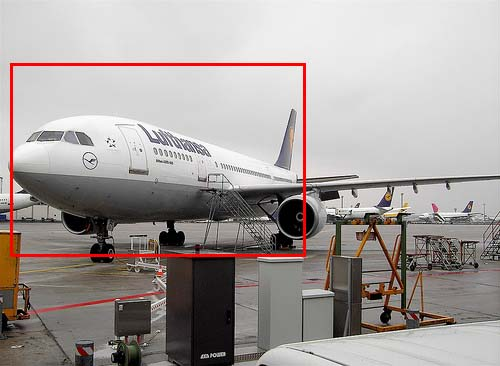
\includegraphics[width=0.8\textwidth]{Figuras/plain.jpg}
   \caption[Región de interés]{Región de interés para un avión. Para un conjunto de imágenes que contienen aviones, las ROI (Regiones de interés), enmarcan las regiones donde se encuentran los objetos pertenecientes a una clase en especifico, lo que se utiliza como ejemplo positivo, logrando separa el contenido que no es el objeto en si mismo, usualmente llamado ejemplos negativos.}
   \label{fig:anota}
\end{figure}

\subsection{Preprocesamiento}\label{subsec:pre}
Una vez creadas todas las anotaciones, se puede iniciar el proceso de creación del modelo. En primera instancia, se agrupan todas las imágenes de acuerdo a la razón entre $w$ (ancho) y $h$ (alto), con lo que se separan los conjuntos de datos en tres partes: datos positivos, es decir, aquellos donde se encuentra el objeto; datos negativos, aquellas imágenes donde no hay presencia de la clase buscada; y finalmente en datos negativos duros, los que contienen imágenes donde hay objetos muy parecidos a simple vista del objeto que estamos buscando clasificar. Finalmente el tamaño de las imágenes será ajustado al promedio de las dimensiones de su razón correspondiente. La estructura del modelo será analizada con mayor detalle en la sección~\ref{sec:model}.

La cantidad de muestras ó tipos de imágenes puede variar influyendo directamente en el resultado, afectando así la efectividad que se haya obtenido en el paso anterior, por lo que es muy importante encontrar y preprocesar un buen conjunto de entrenamiento en una etapa temprana.

\section{Modelo de entrenamiento}\label{sec:model}
Según explica Felzenszwalb et al.~\cite{Felzenszwalb2010}, todos los modelos generados por el marco involucran filtros lineales, los cuales son aplicados a mapas de características densos. De estos mapas se extraen las características más representativas y se crea un vector de características que describe la porción de la imagen que se está observando. A demás, estas características son descritas mediante una variación de HOG el que fue presentado previamente por Dalal and Triggs~\cite{Dalal2005}, aun así el marco de desarrollo es independiente del tipo de extractor de características que se utilice, lo que para nuestro estudio es una ventaja, ya que es aquí donde podemos probar nuestro propio descriptor.

Detalle importante de ese marco de desarrollo son los filtros y sus \textit{scores}, ver Sección~\ref{sec:fas}. La idea es definir un \textit{score} en diferentes posiciones y escalas en una imagen, esto es realizado mediante una pirámide, ver Sección~\ref{sec:pyra}, de características que especifica un mapa de características en un rango fijo.

\subsection{Deformable Part Models}\label{subsec:dpm}
Se definen modelos mediante un filtros raíz que cubre todo el objeto y por filtros de alta resolución que cubren partes más pequeñas del objeto observado. El filtro raíz define la ventana principal para la detección. Los filtros por cada parte del objeto son ubicados $\lambda$ niveles abajo en la pirámide. Las celdas utilizadas en HOG en cada nivel tienen la mitad del tamaño que las celdas del filtro raíz.
Con estos pasos, Felzenszwalb et al.~\cite{Felzenszwalb2010, Felzenszwalb2013} encontraron que los filtros por parte encuentran características más exactas en resoluciones mayores en comparación con un filtro raíz. Por ejemplo, para un rostro, el filtro raíz podría encontrar los bordes de un rostro y los filtros por parte, los ojos, la boca o la nariz.

Formalmente, un modelo con $n$ partes está definido por un conjunto de parámetros $(F_{0}, (F_{1},d_{1}), \dots, (F_{n}, d_{n}), b)$, donde $F_{0}$ es un filtro raíz, $F_{i}$ es una filtro para una parte del objeto, $d_{i}$ es un vector de parámetros de deformación y $b$ es un escalar. El vector $d_{i}$ especifica los coeficientes de una función cuadrática que especifica el costo de una posible posición para un filtro $i$ relativo a la posición del filtro raíz. 

Se genera un hipótesis para un objeto con una vector de configuración $z = (p_{0}, \dots, p_{m})$, donde $p_{i} = (x_{i}, y_{i}, s_{i})$ el que especifica la posición y escala del filtro $i$. El \textit{score} o puntaje de una hipótesis está dado por el \textit{score} de cada parte en su respectiva posición menos un costo de deformación que depende de la posición relativa de cada parte con respecto a la raíz más un escalar de corrección,
\begin{equation}
	\mathit{score}(z) = \sum_{i=0}^n F_{i} \cdot \phi(I, p_{i}) - \sum_{i=1}^{n} d_{i} \cdot \psi(p_{i},p_{0}) + b,
\end{equation} 
$$ \text{donde }\psi(p_i. p_0) = (dx_i, dy_i, dx^{2}_i, dy^{2}_i),$$
$$ \text{con } dx_i = x_i-x_0 \text{ y } dy_i = y_i-y_0$$

El \textit{score} de una hipótesis $z$ puede ser expresado en términos de un producto punto, $\beta \cdot \Phi(I, z)$, entre un vector de parámetros de un modelo $\beta$ y un vector de características $\Phi_z$ según propone Felzenszwalb et al.~\cite{Felzenszwalb2013}.

\subsection{Detección}\label{subsec:detection}
Para detectar un objeto en una imagen se calcula un score general sobre la posición filtro raíz $p_0$ de la imagen de acuerdo al mejor posicionamiento de las partes en relación a $p_0$, 
\begin{equation}	\label{max_score}
	\mathit{score}(p_{0}) = \max_{p_{1}, ..., p_{n}} \mathit{score}(p_{0}, ..., p_{n}).
\end{equation} 

Una detección está definida por un alto \textit{score} de la posición raíz, mientras que  la posición de las partes que cumplen con un \textit{score} alto definen una hipótesis completa de un objeto.

\subsection{Mixture Models}\label{subsec:m_models}
Al existir muchas instancias de una misma clase de objeto, que por ejemplo muestran distintos puntos de vistas, es normal extender la estrategia de tener un modelo por objeto a crear un modelo que mezcle todas esas instancias con el fin de crear un modelo unificado de un objeto, esto recibe el nombre de \textit{Mixture Models}.

Para detectar objetos utilizando \textit{Mixture Models}, primero se calculan los \textit{scores} acumulado de las raíces de forma independiente para cada componente, y luego para cada ubicación del filtro raíz se selecciona la hipótesis del componente de puntuación más alta en ese lugar.

Formalmente, \textit{Mixture Models} está definido como $m$-tuplas, $M = (M_1, \dots, M_m)$, donde $m$ es la cantidad de componentes, es decir $m$ modelos, $M_c$ representa al modelo para el $c$-avo componente. Una hipótesis para un objeto, $z = (c, P_0, \dots, P_{n_c})$ para \textit{Mixture Models} especifica un \textit{Mixture Component}, $1 \leq c \leq m$, y una posición $p_i$ para cada filtro de $M_c$. El \textit{score} o puntaje para esta hipótesis de objeto es el puntaje obtenido por la hipótesis $z^{\prime} = (c, P_0, \dots, P_{n_c})$ para el componente $c$. Al igual que para un modelo simple el \textit{score} de una \textit{Mixture Models} es el producto punto entre el vector de parámetros del modelo y su correspondiente vector de características que depende de la imagen $I$ y una hipótesis $z$.

\section{Latent SVM}\label{sec:lsvmIV}
Los modelos creados por este marco de desarrollo utilizan clasificadores lineales con variables latentes. Para poder entrenar a estos clasificadores se utiliza \textit{Latent} \textit{support} \textit{vector} \textit{machine} \textit{(LSVM)}. Para la creación de LSVM se crea la siguiente función:

\begin{equation}\label{lsvm_f}
f_{\beta}(x) = max_{z \in Z(x)} \beta \cdot \Phi (x, z).
\end{equation} 
Donde $x$ es una entrada, por ejemplo, una ventana de detección; $\beta$ es un vector con los parámetros del modelo; y $z$ son los valores asignados de las variables latentes de una parte posicionada. El conjunto $Z(x)$ define los posibles valores latentes para una muestra $x$.

Como analogía al tradicional SVM, se puede entrenar $\beta$ desde ejemplos etiquetados de la forma $D = (\langle x_1, y_1 \rangle, \dots, \langle x_n, y_n \rangle)$, donde $y_i \in \{-1, 1\}$, minimizando la siguiente función objetivo:
\begin{equation}\label{o_function}
L_D(\beta) = \frac{1}{2} \Vert \beta \Vert^2 + C \sum_{i=1}^n {\rm max} (0, 1-y_if_\beta (x_i)),
\end{equation}
donde ${\rm max} (0, 1-y_if_\beta(x_i))$ representa la función estándar de perdida Hinge y la constante $C$ controla el peso relativo del término de regularización. Dado que el valor de la función~\ref{lsvm_f} es no lineal en $\beta$, la función objetivo~\ref{o_function} de LSVM es no convexa en $\beta$. Sin embargo, el problema de entrenamiento se vuelve convexo una vez la información latente es especificada para los ejemplos de entrenamiento positivos.

Felzenszwalb et al.~\cite{Felzenszwalb2010} explica que $f_{\beta}(x)$ como se define en ~\ref{lsvm_f}, es un máximo de la funciones donde cada una es lineal en $\beta$. Por lo tanto, $f_{\beta}(x)$ es convexa en $\beta$. Esto implica que la función de perdida Hinge es convexa en $\beta$ con $y_i = -1$. Por lo que la función de perdida es convexa en $\beta$ para ejemplos negativos, esta propiedad es llamada \textit{semi-convexidad}.

Debido a esto la función de perdida Hinge en LSVM, no es convexa para ejemplos positivos ya que es el máximo de una función convexa (cero) y una función cóncava $(1-y_if_{\beta}(x_i))$.

Esto es muy importante ya que si consideramos un LSVM donde solo hay un solo valor latente posible para cada ejemplo positivo. En ese caso, $f_{\beta}(x)$ es lineal para un ejemplo positivo y la perdida debido a cada ejemplo positivo es convexa. Combinando esto con la propiedad semi-convexa el resultado se vuelve convexo en $\beta$.

\section{Modelos de entrenamiento}\label{subsec:t_models}

Teniendo un conjunto de imágenes para entrenar, cada una de ellas con sus regiones de interés marcando los objetos de una determinada categoría o clase, por ejemplo, de la clase botella, la región de delimitada será aquella donde se encuentra una botella. Se definen ejemplos positivos por cada una de estas regiones. Estas regiones no especifican etiquetas para los \textit{mixture} \textit{component} o la posición de los filtros, por lo tanto estos son tratados como variables latentes durante el proceso de entrenamiento. 
La información que hay dentro de las regiones se usa para poder posicionar el filtro raíz en cada ejemplo positivo. A su vez se define un conjunto de ejemplos negativos grande, done no hay presencia de los objetos de la categoría que se está analizado.
Por cada posición y escala de una imagen entrega un ejemplo negativo diferente.

El objetivo de separar las imágenes en ejemplos positivos y negativos tiene directa relación con la implementación de LSVM donde la idea principal es obtener un puntaje alto para los ejemplos positivos y un puntaje bajo para los ejemplos negativos, para esto se utiliza el algoritmo presentado en la Sección~\ref{sec:lsvmIV}.

El proceso de entrenamiento consta de varias etapas que a continuación se detallan:

\textbf{Inicialización del filtro raíz}:
Para cada categoría automáticamente se seleccionan las dimensiones del filtro raíz tomando en cuenta el tamaño promedio de las regiones de interés definidas en los datos de entrenamiento. El filtro raíz inicial $F_0$ es entrenado usando SVM normal sin variables latentes. Los ejemplos positivos son extraídos desde el conjunto de ejemplos de entrenamiento sin traslape, es decir donde el objeto es 100\% visible (Estos vienen etiquetados en el conjunto de datos que proporciona PASCAL). Estos ejemplos son re-escalados cuidadosamente al tamaño y razón del filtro. Ventanas aleatorias son creadas en las imágenes negativas para generar ejemplos negativos.

\textbf{Actualización del filtro raíz}:
Teniendo en cuenta el filtro raíz inicial formado en el paso anterior, para región delimitante en el conjunto de entrenamiento se encuentra la mejor puntuación de la posición del filtro que se superpone significativamente con la región de interés definida en los datos de entrenamiento. Esto se hace en la imagen original solamente, en las imágenes creadas no. Luego se re-entrena $F_0$ con el nuevo conjunto positivo y los ejemplos negativos aleatorios, haciendo esto dos veces.

\textbf{Inicialización de las partes}:
En esta etapa se inicializa la cantidad de partes, siendo estas declaradas al momento de inicializar el algoritmo de entrenamiento, Felzenszwalb et al.~\cite{Felzenszwalb2008}, inicializa seis partes desde el filtro entrenado en el paso anterior. Primero, se seleccionan una área $a$ tal que $6a$ sea igual al 80\% del área del filtro raíz. Gradualmente se seleccionan regiones rectangulares de la aréa $a$ del filtro raíz que posee la mayor energía positiva. Los pesos de las regiones se definen en cero y luego se repite el proceso hasta que seis partes son seleccionadas. Los filtros por partes son inicializados con los valores del filtro raíz en la subventana seleccionada por la parte, pero usan relleno para las partes con mayor resolución. Los costos iniciales de la deformación se miden con la norma cuadrada del desplazamiento con $a_i=(0, 0)$ y $b_i=-(1, 1)$.

\textbf{Actualización del modelo}:
Para actualizar el modelo se construyen nuevo datos de entrenamiento, se separan los tres conjuntos de entrenamiento. Para cada región positiva en el conjunto de entrenamiento, se aplica el detector existente en todas las posiciones y escalas con al menos un 50\% de superposición con la región delimitadora dada. Entre esos datos de entrenamiento se seleccionan las posiciones con puntuación más alta en los ejemplos positivos correspondientes a la región delimitada.

Los ejemplos negativos son seleccionados desde las imágenes que no contienen el objeto y entregan un puntuación elevada con la detección. Se añaden los ejemplos negativos a un caché hasta que se llega al límite del tamaño del archivo, esto se declara en un archivo externo de configuración. Un nuevo modelo es entrenado corriendo \textit{SVMLight} en los ejemplos positivos y negativos, cada uno etiquetado con las posiciones de las partes. Se actualiza el modelo 10 veces usando los datos guardados en caché. En cada iteración se guardan los casos difíciles del caché anterior y se añaden tantos nuevos casos complicados como sea posible dentro del límite de la memoria. En las iteraciones finales, podemos incluir todas las instancias de los casos difíciles, en el caché.

\section{Resumen}\label{sec:summaryIV}

En este capítulo se presentó el comportamiento interno del marco de desarrollo creado por el grupo de trabajo de D. Ramanan, el objetivo principal de este capítulo fue presentar las partes principales del marco de desarrollo lo que nos permite poder hacer modificaciones sobre éste, buscando así optimizar su rendimiento y encaminando su desarrollo para poder implementar nuestra propuesta y probarla junto con este programa, para luego comparar los resultados obtenidos. Es de suma importancia presentar este marco de desarrollo ya que es éste programa el que nos ayudara a probar nuestra propuesta con el fin de poder lograr mejoras interesantes.

% Bibliografía
% ---------------------------------------------------------------
% tubiblio.bib es el archivo con la base de datos bibliografica
\backmatter
\bibliographystyle{ieeetr}
\bibliography{referencias}

% Anexos
\appendix
% aca se incluyen los archivos con el texto de los anexos
% (Ej.: anx-uno.tex es el archivo de un anexo)

%==================================================ANEXOS========================================%
\chapter{PRIMER ANEXO}
\label{ch:capIVA}

\lstset{
  basicstyle=\ttfamily,
  columns=fullflexible,
  showstringspaces=false,
  commentstyle=\color{gray}\upshapem,
  language=XML,
  caption={Ejemplo de anotación, Archivo XML que contiene la estructura de una anotación},
  label=AnotacionXml
}
\begin{lstlisting}[frame=single][tb]
<annotation>
	<folder>VOC2011</folder>
	<filename>2007_000033.jpg</filename>
	<source>
		<database>The VOC2007 Database</database>
		<annotation>PASCAL VOC2007</annotation>
		<image>flickr</image>
	</source>
	<size>
		<width>500</width>
		<height>366</height>
		<depth>3</depth>
	</size>
	<segmented>1</segmented>
	<object>
		<name>aeroplane</name>
		<pose>Unspecified</pose>
		<truncated>0</truncated>
		<difficult>0</difficult>
		<bndbox>
			<xmin>9</xmin>
			<ymin>107</ymin>
			<xmax>499</xmax>
			<ymax>263</ymax>
		</bndbox>
	</object>
	<object>
		<name>aeroplane</name>
		<pose>Left</pose>
		<truncated>0</truncated>
		<difficult>0</difficult>
		<bndbox>
			<xmin>421</xmin>
			<ymin>200</ymin>
			<xmax>482</xmax>
			<ymax>226</ymax>
		</bndbox>
	</object>
	<object>
		<name>aeroplane</name>
		<pose>Left</pose>
		<truncated>1</truncated>
		<difficult>0</difficult>
		<bndbox>
			<xmin>325</xmin>
			<ymin>188</ymin>
			<xmax>411</xmax>
			<ymax>223</ymax>
		</bndbox>
	</object>
</annotation>

\end{lstlisting}


%\chapter{SEGUNDO ANEXO}
%\label{ch:capituloAB}
%
%
%Contenido del segundo anexo.



% ... mas archivos de anexos

\end{document}
% ---------------------------------------------------------------